\documentclass[11pt,onecolumn]{article}

\usepackage{url}
\usepackage[colorlinks=true,citecolor=blue]{hyperref}
\usepackage{amsmath,amsfonts,amssymb,mhchem,chemfig}
\usepackage{cases}
\usepackage{setspace}
\usepackage{caption}
\usepackage{textgreek}
\usepackage{authblk}
\usepackage{natbib}
\usepackage[margin=0.75in]{geometry}
\usepackage[margin=0.5in]{caption}
\captionsetup[figure]{font=footnotesize,labelfont=footnotesize}
\pagestyle{plain}
\bibliographystyle{abbrvnat}
\setcitestyle{authoryear,open={(},close={)}}
\providecommand{\keywords}[1]{\textbf{\textit{Key words---}} #1}
\renewcommand{\abstract}[1]{\textbf{Abstract --- } #1}
\newcommand{\vect}[1]{\boldsymbol{#1}}
%\jshort{mst}

%\volname{}

%\jvolume{0}

%\jvol{}

%\jissue{0}

%\pubyear{2020}

%\mstype{Article}

%\artid{012}

%\access{}
\renewcommand{\baselinestretch}{1.45} 

%\captionsetup{font={stretch=3}}
\newcommand{\othercaption}[1]{\caption{\setlength{\baselineskip}{1.5\baselineskip}#1}}

\begin{document}

\title{High order epistasis, Complexity and mutation-selection-drift balance: insights from a mechanistic approach}
\date{\today}
\author[,1]{Florian Labourel\thanks{Corresponding author: \texttt{florian.labourel@univ-lyon1.fr}}}

 
\affil[1]{Univ Lyon, Université Lyon 1, CNRS,
    Laboratoire de Biométrie et Biologie Evolutive UMR5558,
    F-69622 Villeurbanne, France}

  \maketitle
    
    \abstract{Epistasis is a pervasive phenomenon tightly linked with the complexity of biological systems that both influence trajectories followed by Evolution and its steady-state. However, the specific role played by complex high dimensional epistatic relationships in the establishment of evolutionary steady-state has mostly remained a conundrum up until now. Here, we put forward a new kind of epistasis - namely complementary epistasis - and shows how this improvement based on mechanistic considerations may change some predictions about mutation-selection-drift balance, and, in turn, help interpret genomic data. We argue that this idea seems well-suited to be studied analytically within a theoretical population genetics framework that remains to be developed in that sense, which would be the first part of this project. We then discuss how this idea can be further explored and how it could broaden our theoretical knowledge on both general and more specific questions in evolutionary and molecular biology. To illustrate this, we then focus on the phenotypic evolution of proteins, especially enzymes, to demonstrate that it cannot be fully understood without this new framework due to their embedding in metabolic pathways. Such a study would be the second part of the project. Finally, we argue that combined with other biological considerations, enriching the framework could also help make predictions about molecular evolution, which would be one of the several possible extension to this project.}

\keywords{Complementary epistasis, global epistasis, mutation-selection-drift balance, complexity, modularity, neutral evolution, protein evolution, molecular evolution}
\vspace{0.5cm}

\pagebreak

\section{{Introduction}\label{sec:Intro}}

‘‘\textit{The limits of my language are the limits of my world}''.

\citep{Wittgenstein22}

Evolution is the ongoing process that gave birth to the wide zoo of organisms that have ever lived and shall ever live \citep{Darwin59,Wallace58}. It is, as it were, the language of Nature when it deals with mutable self-replicating entities. If this language has been fruitful, it still sets the limits of what can exist and how this space of possibilities is explored, as pinpointed by \citet{Wittgenstein22}. Melting many mechanisms acting at different levels of space and time, these limits are yet to be fully understood. It has long been known indeed that the power of Natural Selection is limited by genetic drift \citep{Wright30} such that organisms are the best of the possible ones under the conflicting mutational and selective pressures \citep{Kimura62,Ohta92}, but how it combines with the complex genetics underlying traits remains, to say the least, inchoate.\\

Epistasis\footnote{see Glossary at the end of this document for further details on the different kind of genetic interactions with a specific focus on epistasis ones.} is a ubiquitous phenomenon in which the effect of a mutation differs depending on the genetic background in which it occurs \citep{Bateson09,Phillips08}. As \citet{Weinreich13} pointed out, it is a measure of our ‘‘surprise" insofar as we \textit{a priori} expect mutational effects to be additive \citep{Phillips08}. Epistasis has long been known to occur between pairwise mutations where the combined effect between them results in a phenotype or a fitness that is not the sum of that they would have in isolation from one another: if Adaptation can still occur through few genetic changes \citep{Orr05}, such epistatic interactions in general comes with several consequences, narrowing the paths towards adaptation \citep{Poelwijk07} for instance, and could also create fitness valleys under certain circumstances called reciprocal sign epistasis \citep{Weinreich05b,Poelwijk11}.

Because of the process of genetic drift \citep{Wright30,Kimura58,Ohta92} that entails a mutational load \citep{Haldane37,Muller50,Agrawal12}, it was thus supposed that small effective population sizes could help escape from a local fitness peak by facilitating fixation of intermediate deleterious mutations \citep{Wright30,Wright32}; therefore, subdivision in small populations should be better at finding the highest peak though they are less efficient to climb up to this peak. However, introducing polymorphism and recombination disproved this conclusion \citep{Weinreich05} since combined mutations can either be found through stochastic tunneling \citep{Iwasa04b} or be brought together after having emerged in different lineages, and it was later shown that considering the width -- \textit{i.e.} the number of loci making up the valley -- of valleys would even reverse Wright's initial intuition with higher populations more prone to cross large fitness valleys, especially if these valleys are much alike plateaus \citep{Weissman09}.

Known as higher-order epistasis, this phenomenon involving many loci usually gives rise to rugged fitness landscapes \citep{Kauffman87,Kauffman89,Weinreich13} where peaks and valleys quickly follow each other in both the phenotype and the genotype spaces. Based on the NK-model, \citet{Kauffman87} shown that complexity -- in terms of complex epistasis relationships which may exist between nucleotides, genes, pathways, or even organisms subunits such as organs -- comes at a great cost for fitness since more ruggedness in turn increases the probability of being trapped on a local optimum \citep{Kauffman87,Geard02}, a finding which was further confirmed when accounting for the possibility of neutral mutations, through NKq and NKp models \citep{Barnett98,Newman98,Geard02}. Under certain assumptions, this model makes possible to estimate analytically the average expected mutation-selection-drift balance \citep{Weinberger91}, which can be contrasted to other such predictive frameworks.

Indeed, the influence of complexity on evolutionary trajectories has in parallel thoroughly been addressed through the lens of Fisher's geometrical model \citep{Fisher30,Orr98,Orr00,Martin06,Tenaillon07,Tenaillon14} where epistasis builds up from the mathematical underpinnings on which the framework relies \citep{Hartl96,Orr00,Tenaillon14} and the assumption of pleiotropy preexistence \citep{Tenaillon14} - see \citep{Stearns10} for a review on pleiotropy. Besides enabling to study the distribution of fitness effects \citep{Martin06,Lourenco11}, it is in principle possible through this framework to approach how complexity -- in a broad sense covering independent phenotypic traits, epistasis, pleiotropy among other (and more organismic) features -- emerges and evolves \citep{Orr98,Martin07,Gros09,Le-Nagard11}, what it really portrays and even to try and derive that of an organism from the strength of drift an organism experiences \citep{Tenaillon07}. This is because epistasis and pleiotropy are intrinsic features to the multidimensional formulation of the model \citep{Tenaillon14} such that complexity needs not be defined in terms of the unknown explicit genotypic-phenotypic relationships, but can on the contrary be understood as the factor limiting the strength of selection when adopting a top-down approach \citep{Le-Nagard11}.\\

Though fascinating, both these frameworks lack a mechanistic basis as highlighted recently by \citet{Martin14} and \citet{Yi19} -- even if Fisher's geometrical model was specifically revived for this purpose by \citet{Hartl96} and subsequently led to several insights \citep{Martin06,Martin07} -- and, at least, deserves to be informed by the very biological processes giving rise to epistasis and pleiotropy if we are to succesfully achieve a functional synthesis \citep{Dean07} that enables one to disentangle causes from effects in Evolution. For instance, it has been shown that the distribution of fitness effects can be captured using such models \citep{Martin06,Huber17}, but how alternate and potentially more parsimonious explanations could account for similar patterns is largely unknown \citep{Lourenco11}. In the same vein, determining how features such as modularity \citep{Wagner07,Segre05,Hartwell99} changes the landscape and whether it is a specific kind of intrinsic interactions or the evolutionary product these interactions favours or even made necessary requires to understand how they all dynamically behave together, as was argued for molecular networks \citep{Alexander09}.

This is especially significant inasmuch as the genotype-phenotype-fitness map stems from the intertwining between interacting genes - susceptible to evolve \citep{Gros09} during the course of Adaptation - with their basic and emerging physiochemical properties \citep{Bershtein17}. \citet{Yi19} proposed that, contrary to \citet{Dobzhansky73}'s view, ‘‘nothing in Evolution makes sense except in the light of Biology", which rightly questioned the original statement and rejuvenated the debate on the influence of mechanisms and constraints \citep{Gould79}, but failed to avoid circular reasoning. In fact, since Biology is the product of the joint Evolution of physical entities whose combined properties are explored in a (non-random) particular way \citep{Monod71,Monod74,Wagner12} during the process, it seems more likely that \citet{Dobzhansky73}'s statement holds if and only if we acknowledge that nothing in Evolution makes sense without accounting for physics and chemistry, which raises the need for more investigation merging these fields \citep{Dean07,Serohijos14}. Lately, shy first steps to fill in this theoretical gap have adopted the paradigm of statistical physics in an interesting attempt to derive the isotropic instance of Fisher's geometrical model from first principles \citep{Martin14}, drawing inspiration from results of systems biology such as those of the FBA (Flux Balance Analysis) \citep{Orth10}, which, for several reasons\footnote{First, FBA relies on an assumption of optimality to solve the systems of equations describing the process as well as on the existence of fixed molecule contents. Yet more importantly, because this framework does not deal with real mechanisms but only describes a complex system that has already evolved, it cannot explain why nor how it evolved the way it did.} should however not be the appropriate framework to study Evolution - see for example \cite{Schuster08}.

To our knowledge, it has not yet been determined how the combination of complementary epistasis -- where a phenotypic trait can only be competitive if each and any of its underlying loci are (see Figure \ref{fig:ComplementaryEpi} for more details) -- with global epistasis could specifically change population genetics predictions arising from the Neutral Theory of Evolution and its extensions \citep{Kimura68,Ohta73,Ohta92} while this process seems to be supported by mechanistic underpinnings \citep{Kacser73,Hartl85,Yi19,Taverna02,Bloom05,Labourel20}. This is what we propose to do in this project; to justify the interest of such an investigation, we start with the presentation of a toy model based on simplistic assumptions from global epistasis. We then show how this framework may have a profound impact on our understanding of Evolution at different levels of biological organization and put forward the key components that a more complete instance of the model should include. Finally, we introduce how it can be tested and applied by contrasting its results to those obtained when simulating enzyme evolution along one and/or multiple pathways, and conclude by discussing possible further developments, among which the link with protein stability and evolutionary rates are of particular interest as well as the influence of stochastic environments on the actual coefficient of selection.

\begin{figure}[h!]
    \centering
    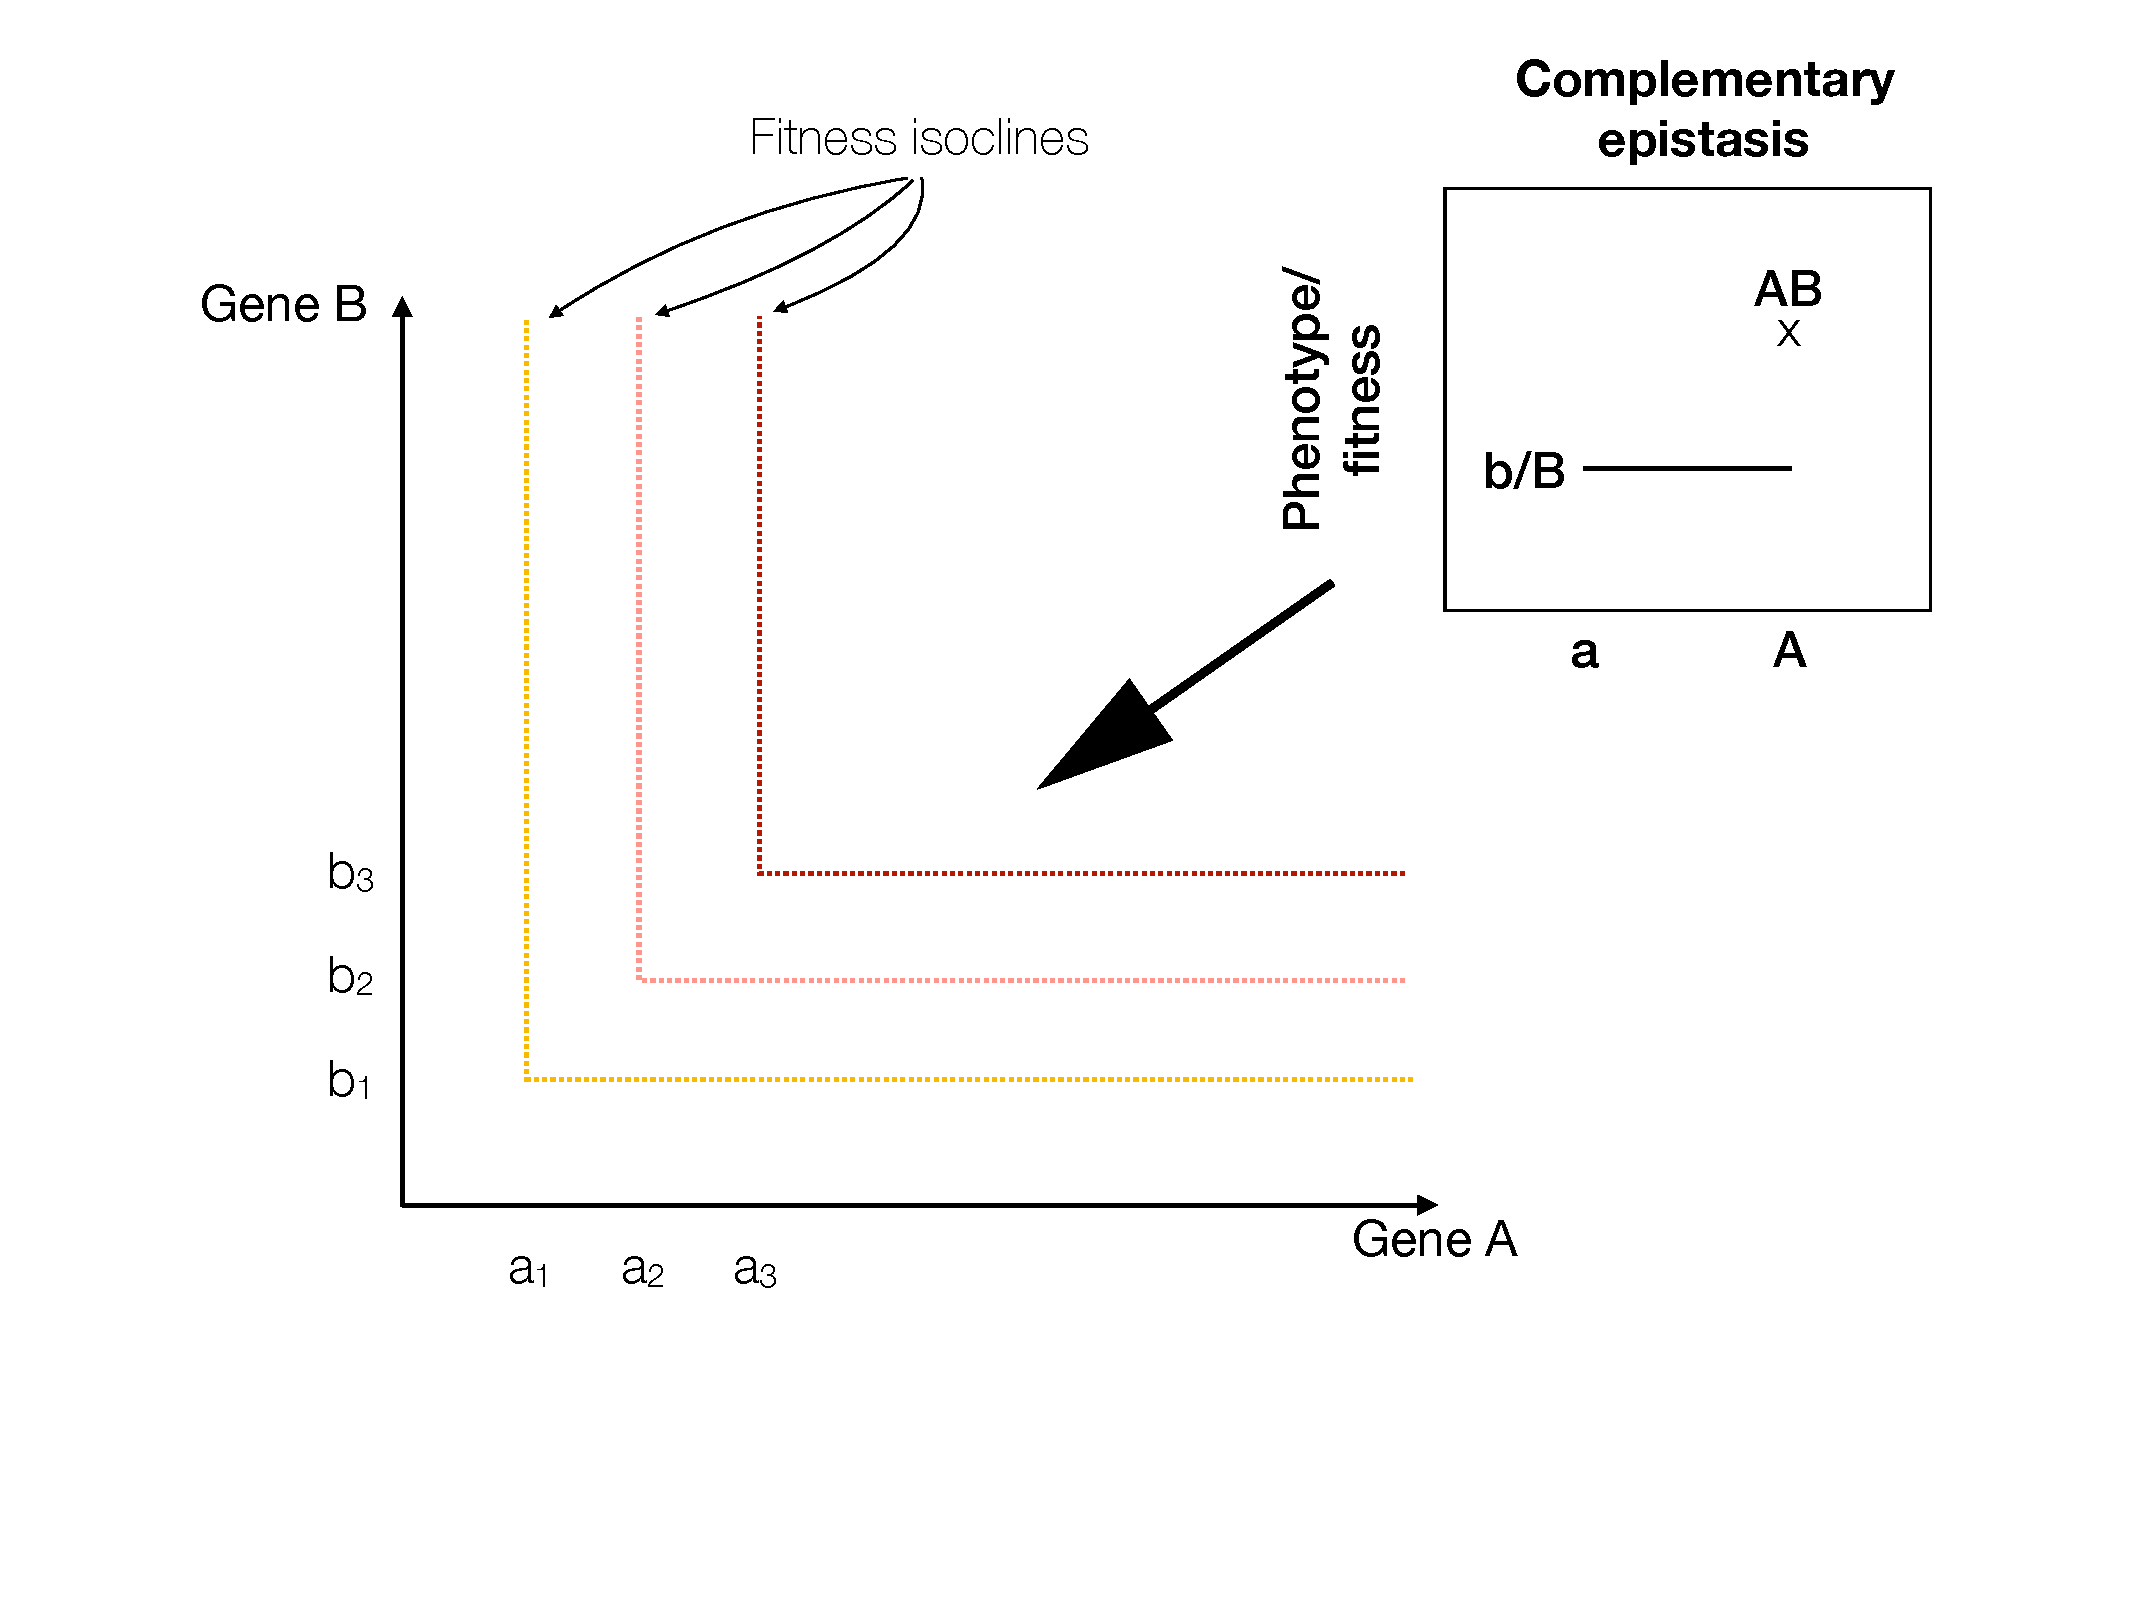
\includegraphics[scale=0.3,trim=3.2cm 4cm 3.2cm 1cm,clip]{Complementary epistasis.pdf}
    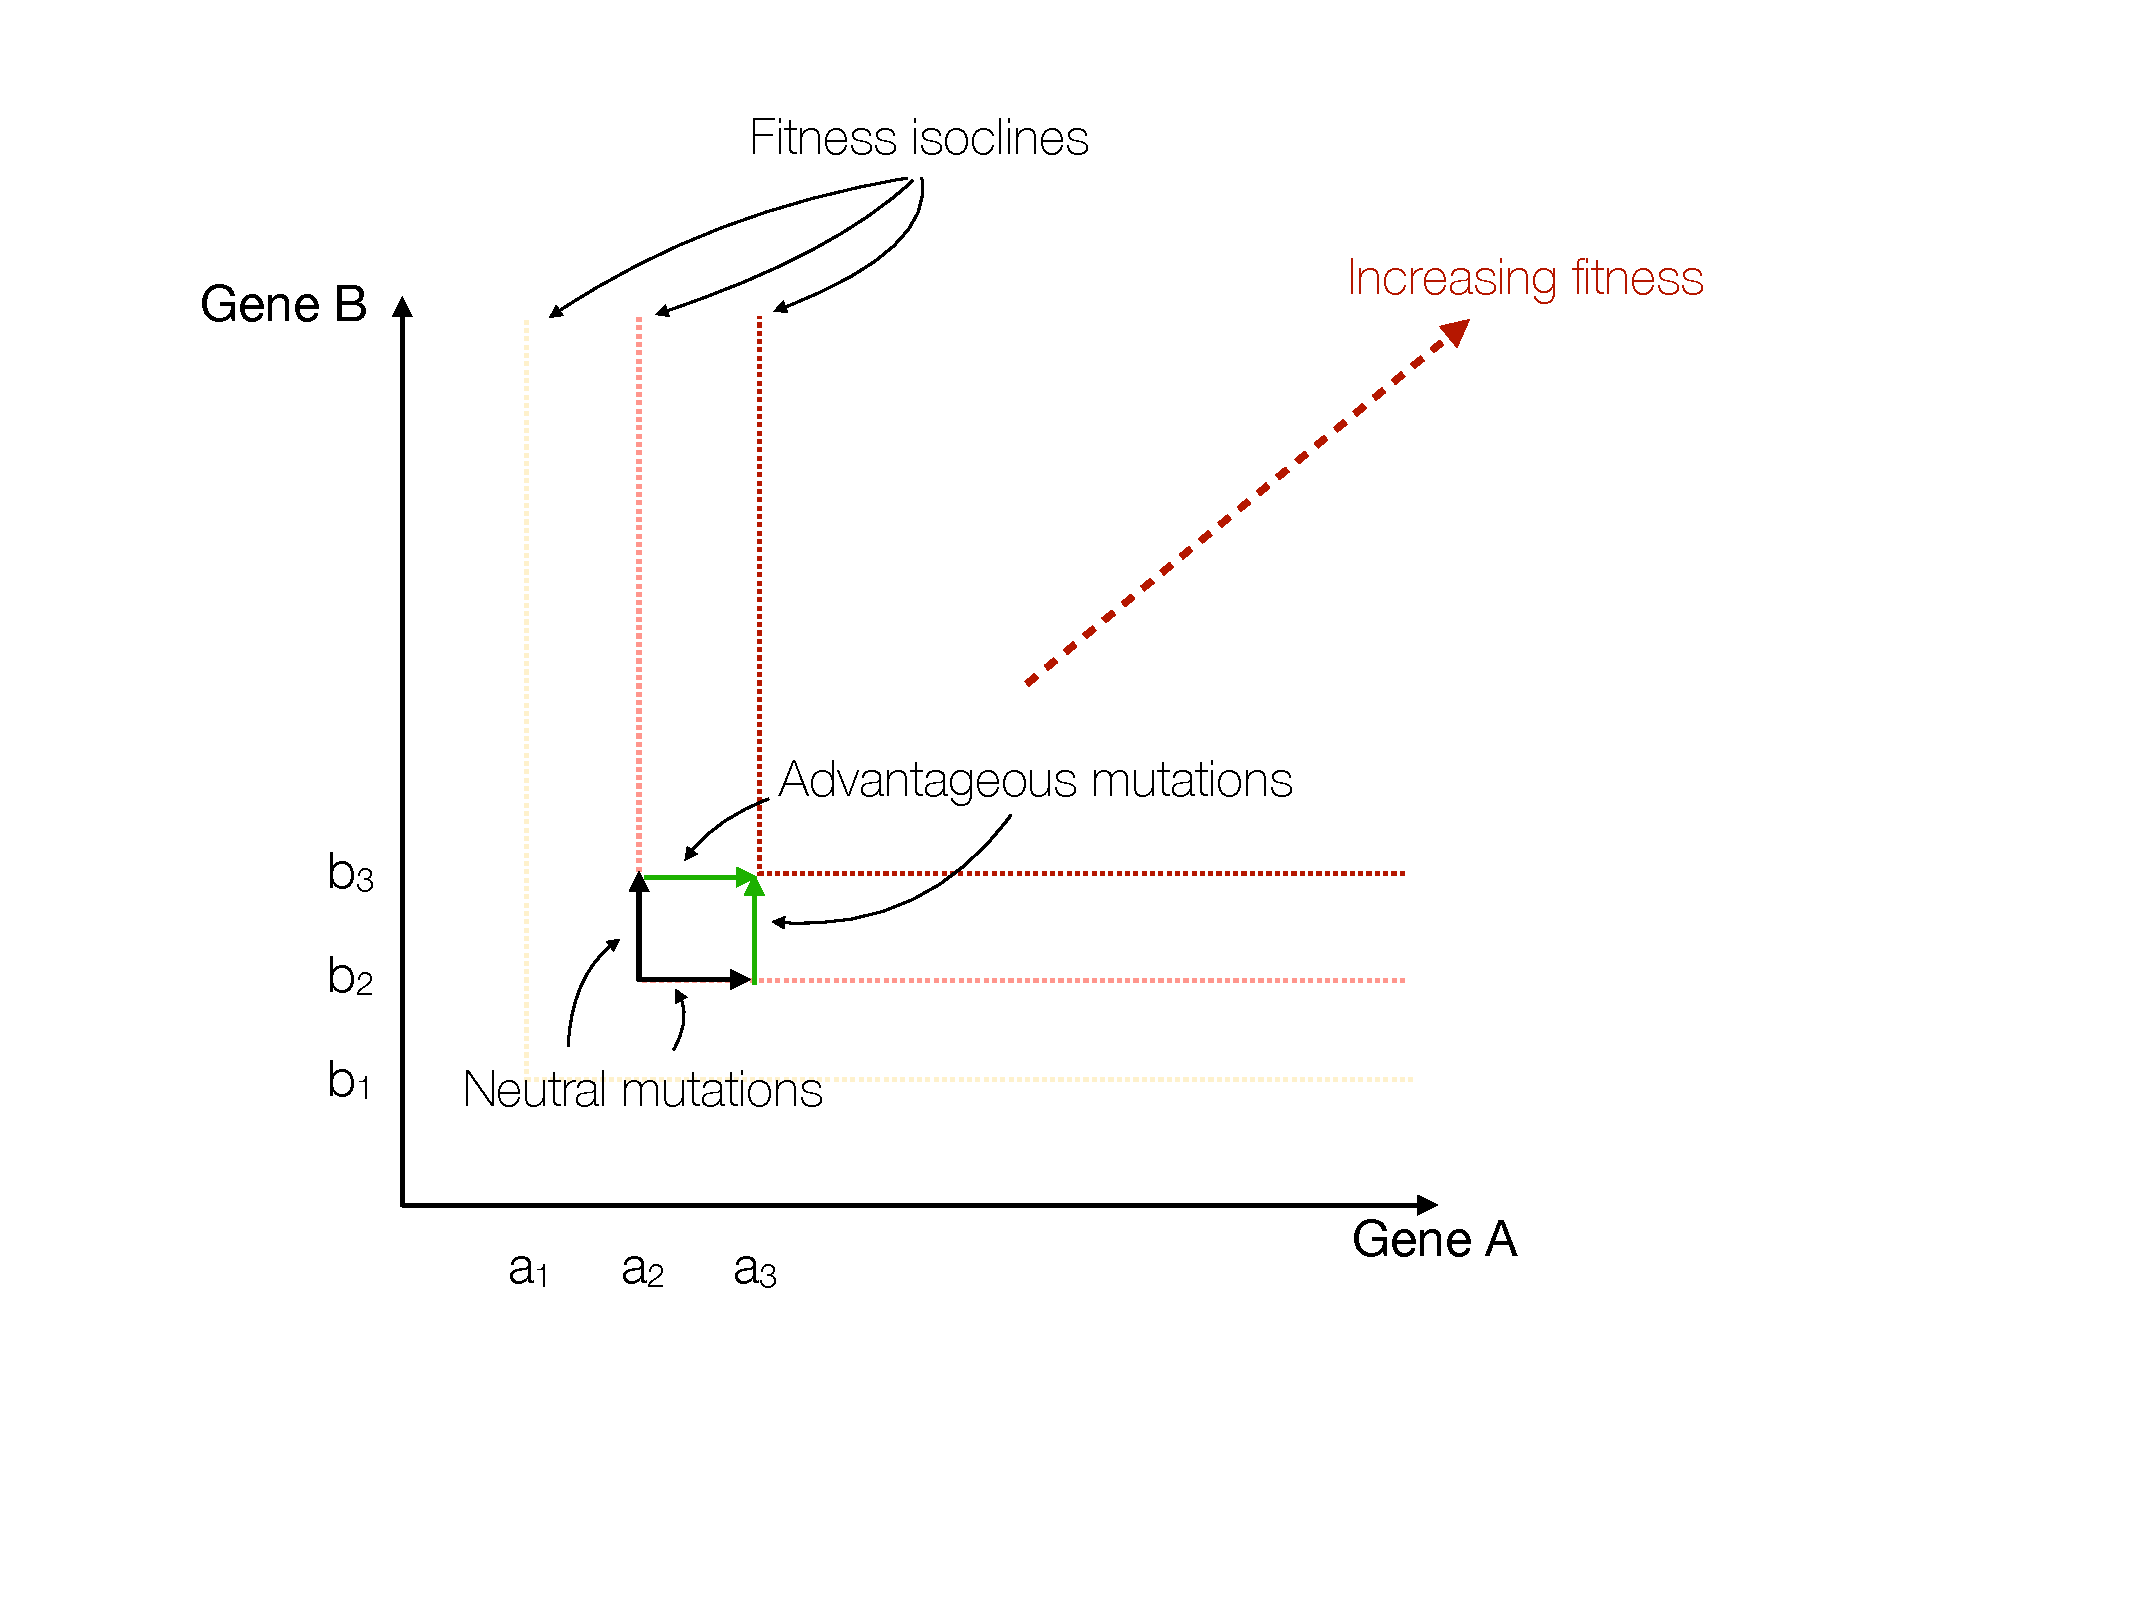
\includegraphics[scale=0.3,trim=3.2cm 4cm 6cm 1cm,clip]{Complementary epistasis_EvoTraj.pdf}
    \caption{Description of complementary epistasis: on the left panel, its effect in the classical a/A-b/B case is shown in the short window, with the need for both A and B mutations to experience any gain of fitness, while the larger plot represents how phenotype/fitness isoclines can be mapped in the genotype space when more mutations are considered. On the right panel is shown the mutational path that allows to gain an extra fitness: first, a potentially advantageous but actually perfectly neutral mutation needs - at least - to exist on either one of the locus before the advantageous mutation can occur and give an actual extra push of fitness. This phenomenon can involve higher order interactions leading to the need for the segregation of numerous neutral mutations which may be subject to mutational biases.}
    \label{fig:ComplementaryEpi}
\end{figure}



\section{{A first approach}\label{sec:FA}}

\subsection{Prediction}

We expect that complementary epistasis should influence both the speed of selection, as was observed for evolutionary escape \citep{Weinreich05,Weissman09} and the mutation-selection-drift balance (see introduction for previous approaches on this idea), and focus on this latter phenomenon. More particularly, we assume that fitness should decrease with the number of genes/loci involved and that the mutational bias should play a large part in limiting adaptation because it influences the preexistence of potentially complementary beneficial mutations (at loci which are drifting because there differ from the worst one). Nevertheless, it should be possible to derive a prediction from the underlying premises of such a phenomenon.

Based on results of the neutral theory of Evolution \citep{Kimura62,Ohta73}, we indeed know that Natural Selection cannot filter mutations whose selective effect $|s|$ is below $1/N_e$. If fitness is limited by a maximum value, this means that deleterious mutations with effects $|s|\approx 1/N_e$ evolve through genetic drift and that fitness at the mutation-selection-drift balance establishes around $\widetilde{f_1}\approx 1-1/N_e$ when mutations are mostly deleterious and one locus is considered \citep{Kimura58}. Let us say that an organism starts with the maximum possible fitness. Through drift on the first gene, $f$ should decrease on average to approximately $1-1/N_e$. Drift on the second gene should again push fitness downwards since the maximum fitness relatively to which drift occurs is now set to $1-1/N_e$, such that $\widetilde{f_2}\approx (1-1/N_e)\times (1-1/N_e)=(1-1/N_e)^2$. Therefore, considering $n$ complementary genes yield the following prediction $\widetilde{f_n}\approx (1-1/N_e)^n$. If $N_e>>1$, this can be summarized by $\widetilde{f_n}\approx 1-n/N_e$. This rough estimate is very similar to that from the Fisher's geometrical model in a N-dimensional space \citep{Hartl96,Poon00} that considers the influence of complexity on the evolutionary equilibrium.%through patterns of pleiotropy and epistasis emerging from the underlying assumptions of the model \citep{Tenaillon14}.

\subsection{Toy model}

In this toy model, we consider a fitness landscape subject to saturation due to diminishing returns epistasis \citep{Tokuriki12,Kaltenbach14} as has widely been documented for proteins in the case of stability \citep{Taverna02,Bloom05,Bloom06,Kaltenbach14} and catalytic efficiency \citep{Dykhuizen87,Hartl85,Yi19,Labourel20}. It has also been recently shown that global diminishing returns epistasis \citep{Kryazhimskiy14,Bahcall14,Otwinowski18} should arise for a complex trait as a by-product of the distribution of fitness effects \citep{Reddy20}. Such a fitness landscape is typically describe through a S-shaped function whose shape is given by the following equation (similar to that of Michaelis Menten):
\begin{align}
    f(x)=\frac{x}{x+K_X}
    \label{eq_sat}
\end{align}The evolutionary process is simulated using the probability of fixation \citep{McCandlish14}, which is a classical result in population genetics \citep{Haldane27,Kimura62,Wright31}. Under this assumption, the probability that a mutation occurring in a haploid population is eventually fixed is given by:
\begin{align}
    P_{\text{fix}}(s,N_e)=\frac{1-e^{-2s}}{1-e^{-2N_es}}(\approx \frac{2s}{1-e^{-2N_es}} \text{, when $s<<1$})
\end{align}
 Let us say that $\vect{X}$ is the vector representing a state of the pool of complementary genes\footnote{For convenience, we only mention genes, but as stated previously, it may also apply to loci or organismic units, for instance.} where  $X_i$ denotes the phenotypic value of any gene $(i)$, and that $s_m'=\frac{f(X_m')-f(X_m)}{f(X_m)}$ denotes the potential selective value of a mutation with fitness $f(X_m')$ occurring on the gene $(m)$. The fitness function detailed above determines the maximum fitness a gene can potentially induce (\textit{e.g.} the maximum catalytic flux an enzyme may be able to sustain). Owing to the specific process of complementary epistasis, the fate of a mutation is decided by the genomic background in which it occurs since it changes the selective effect it provides to its carrier. Two cases have to be distinguished, as we detailed below.
 
 First, if the mutation affects the less efficient gene of a pool of complementary genes -- \textit{i.e.} $X_{m}=\min \limits_{i \in S_g} X_i$ such that $f_{\vect{X}}=f(X_m)$, with $S_g$ the set of genes involved in the phenotypic set $\vect{X}$ -- the probability of fixation of the mutation $X_m'$ rises only up to the threshold where it is no longer the worst gene of the pool. It yields:
 \begin{align}
     P_{\text{fix},X_{m}'} = \left\{
    \begin{array}{ll}
        P_{\text{fix}}(s_m',N_e)\text{, when $s_m'$} \leq \Delta s_{max,m} \\
        P_{\text{fix}}(\Delta s_{max,m},N_e)\text{, otherwise,}
    \end{array}
\right.
\label{eq:Pfix_compepi1}
 \end{align}
 
where $\Delta s_{max,m}=\min \limits_{\substack{i \in S_g \\ i\neq m}} \frac{f(X_i)}{f(X_m)} - 1$ (with $\Delta s_{max,m} \geq 0$). 

Conversely, if the mutation influences the phenotypic value of any other gene -- \textit{i.e.} $X_{m}>\min \limits_{i \in S_g} X_i$, with $S_g$ the set of genes involved in the phenotype $\vect{X}$ -- its probability of fixation is that of a perfectly neutral mutation as long as the phenotypic value for this gene remains above the minimum of the set while it is that of a disadvantageous mutation -- relatively to this threshold -- when it falls under it, such that:
 \begin{align}
     P_{\text{fix},X_{m}'} = \left\{
    \begin{array}{ll}
        1/N_e\text{, when $s_m'$} \geq \Delta s_{min,m} \\
        P_{\text{fix}}(s_{act,m'},N_e)\text{, otherwise,}
    \end{array}
\right.
\label{eq:Pfix_compepi2}
 \end{align}
 
where $\Delta s_{min,m}=\min \limits_{\substack{i \in S_g}} \frac{f(X_i)}{f(X_m)} - 1$ (with $\Delta s_{min,m} \leq 0$) and $s_{act,m'}=\frac{f(X_m')}{\min \limits_{\substack{i \in S_g}} f(X_i)}-1$. 

Within such a framework, the actual selective advantage of a mutation is largely dependent on the worst loci in the set; as a corollary, it does not depend on the phenotypic value of the focal locus. One should notice that neither clonal interference nor double/multiple mutants are considered, meaning that the fixation process concerns only one mutation (on one gene) at a time.

Finally, we tested the influence of different distribution of fitness effects ranging from cases with no mutational biases ($b=0$) to some with high ones ($|b|=\lambda X_m$, where $\lambda>>0$). To comply with estimates on biological phenotypic traits  be they catalytic constants \citep{Carlin16} or gene expression \citep{Metzger16,Hodgins-Davis19}, the distribution of mutational phenotypic effects is modelled through a Gaussian distribution whose mean depends on the present value of the trait $X_m$ at the loci $m$, a mutational bias $b$ pushing the trait value downwards and a variance $\sigma_X^2$ of the fitness effects of mutants. Both because it seems more realistic \citep{Carlin16} and because the optimization process would otherwise be far longer, mutations are drawn for the $log_{10}$ value of the trait such that mutations affecting higher phenotypic values have a proportionally higher variability and are more biased (when the bias is not null). This can be summed up by the following mutational distribution, in which $X_m'$ is drawn:
\begin{align}
log_{10}(X_m') \sim \mathcal{N}(log_{10}(X_m)-b,\sigma)
\end{align}

Note that there exists a broad scientific literature on the distribution of fitness effects of mutations \citep{Keightley07,Orr03,Gillespie84} and some previous theoretical hypothesis for it (see for instance \cite{Martin06} and \cite{Rice15}), but we are here interested in the making of these effects from underlying causes and cannot, as a consequence, use distributions that result from the phenotype-fitness map. We shall later discuss this point as a direct perspective of the present project.

\subsection{Simulation and results}

\begin{figure}[h!]
    \centering
    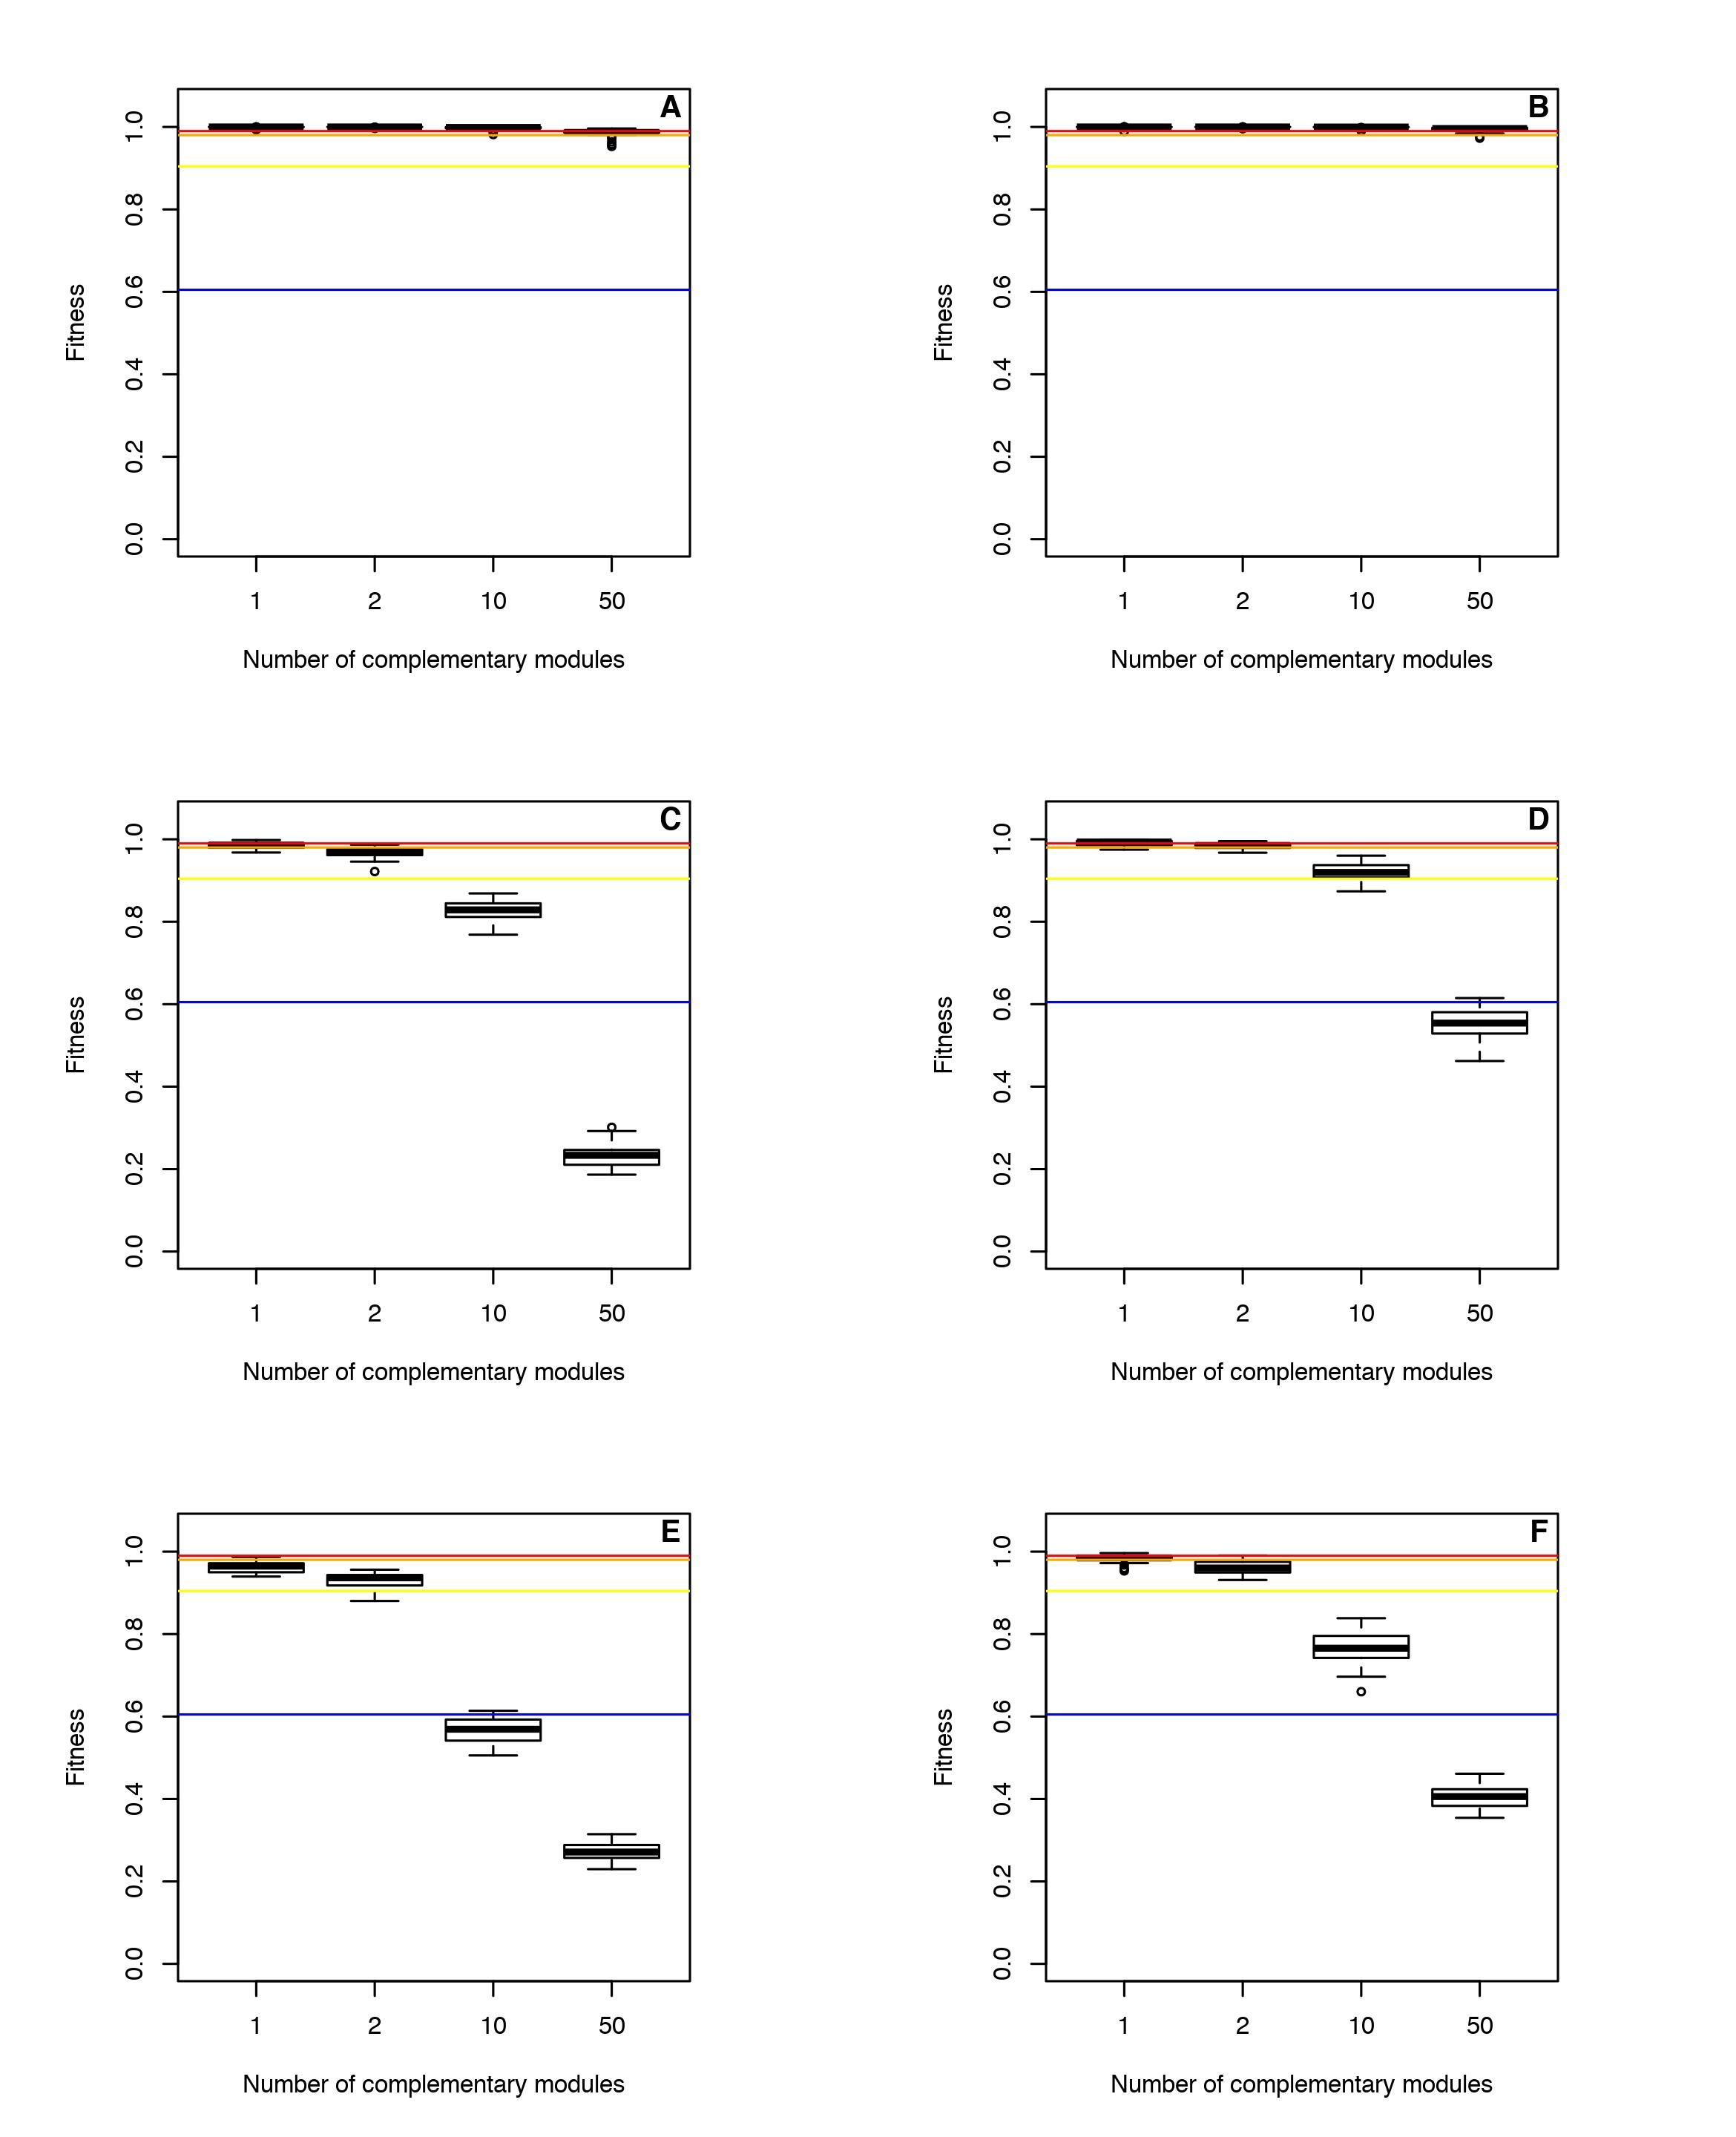
\includegraphics[scale=0.75,trim=0cm 0cm 0cm 0cm,clip]{Evo_Outcomes_Ne100.jpeg}
    \caption{Simulation outcomes for the mutation-selection-drift balance with $N_e=10^2$ when the interplay of complementary epistasis and diminishing returns epistasis (through the fitness landscape of traits) are accounted for. The number of complementary modules (\textit{eg.} genes) varies from 1 to 50. Each line corresponds to a level of mutational bias: null in (A) and (B), low in (C) and (D), high in (E) and (F) - see text for details; each column represents a level of mutational variability, with (A), (C) and (E) having low variability while (B), (D) and (F) display a moderately high variability.}
    \label{fig:Outcomes100}
\end{figure}

In order to demonstrate the relevance of studying this phenomenon, we tested as a premise the influence of complementary epistasis on the mutation-selection-drift balance. To do so, we set $K_X=1$ in equation (\ref{eq_sat}). Three mutational biases were considered ($0$;$-\sigma_X$;$-2\sigma_X$) ranging from no bias to a high one through which only 1 mutations out of 40, approximately, is advantageous. We also studied two different levels of phenotypic variability among mutants for the $log_{10}$ of $X_m'$ ($\sigma_X=0.25$ and $\sigma_X=0.5$), with the highest one producing advantageous mutations with greater selective effects while decreasing the relative pool of slightly deleterious ones. These sets of parameters are in line with the aforementioned estimates for the distribution of phenotypic effects of mutations \citep{Carlin16,Metzger16}. The initial value of each complementary phenotypic trait was set to $X_0=1-1/N_e$ to start from the null hypothesis of nearly-neutral Evolution. Finally, the probability of fixation was computed through either equation (\ref{eq:Pfix_compepi1}) or equation (\ref{eq:Pfix_compepi2}) depending on the locus which was affected and the simulations were ran for an average of $1000$ mutation events per gene.

We simulated the evolutionary process for $N_e=10$ (see APPENDIX section at the end) and $N_e=100$ and present results obtained for the mutation-selection-drift balance in this latter case. In line with expectations, we observe that the number of complementary genes (denoted under the generic term of modules in the figure) severely impairs the strength of Natural Selection, with a decrease more or less of the order of $N_{mod}\times 1/N_e$ when mutational biases are considered. However, this is not the case when no bias is considered with a decrease being far more limited that does not jeopardise the optimisation process albeit marginally - see (A) and (B) on Figure (\ref{fig:Outcomes100}). Because deviations from the expected equilibrium can accumulate, the balance is also more sensitive to the variability of mutational effects, with lower variability coming with a predictable decreased fitness - due to an increased amount of slightly deleterious mutations and a decreased amount of largely advantageous mutations - for the same level of mutational bias (compare (C) and (E) with (D) and (F) on Figure (\ref{fig:Outcomes100})). Owing to the very low effective population sizes, drift overwhelms Natural Selection and pushes the balance towards very low values, a process already documented in models based on universal pleiotropy such as \citep{Hartl96} and \citep{Poon00}. But we show here using a toy model that such complexity-selection trade-off may be readily observed without any preexisting pleiotropic relationship (and without accounting for the decrease of effective population size usually associated with complexity), and lends credit to the idea of an intrinsic cost to complexity.

\subsection{Consequences and perspectives for this project}

Obviously, there is a need to study higher and more realistic population sizes in order to draw robust conclusions. But, because the aim of this new framework is to try and understand the influence of epistasis from physical and chemical first principles, it definitely also needs include other relevant features that should influence evolutionary outcomes. First, it is known that mutations occurring on coding sequences, even being synonymous, are rarely exactly neutral, reflecting in particular the cost arising from codon usage bias \citep{Ikemura85,Galtier18,laBella19}. In parallel, not all kind of phenotypic trait undergo deleterious mutational biases: this is especially true for levels of expression\footnote{And organic shapes, albeit for different reasons.},  which result from changes in gene networks features such as the level of trans-regulatory elements, their specificity and a complex pleitropic set of relations with cis-regulatory elements \citep{Hodgkin98,Chesmore16} involving the whole genome. Last but not least, if biological systems may be thought to be under directional selection to maximize growth and biomolecules production, the intertwining of pathways and biological reactions is more likely to result in a slightly different picture than that displayed by a simple positive complementary epistasis : genes that are too efficient may at some point yield collateral damages either because they monopolize resources in vain or induce toxicity (\textit{eg.} producing too many metabolites) \citep{Lilja17,Niehaus20,Labourel20}. Consequently, it seems more realistic that each of the non-worst genes is under more or less relaxed stabilizing selection towards an optimum, coinciding with the worst gene  -  that can only change when the worst gene of the set improves to a higher value - which means that even when no mutational bias exists, most genes involved in complementary epistasis should be pulled towards the worst one, for complementary epistasis becomes negative in those cases.

Being directly based on functional insights, such a framework seems very relevant to start tackling the challenges set out by the joint evolution between basic functional epistasis -- and more broadly, genetic interactions -- and Adaptation from a population genetics theoretical perspective. In spite of its apparent specificity, it can indeed describe both intra-level and multilevel evolution: it is appropriate to describe the joint evolution of organs/appendages, as well as enzymes along a pathway, or organs/appendages and enzymes all together, provided that one knows how the genotype-phenoype-fitness map builds up. A first step of the project would therefore aim to deal analytically with simple instances of this model\footnote{Fisher's geometric model or Kaufman's NK complexity model seem well suited to feed into the thinking, but at this stage, it is not possible to state if they can properly translate the model assumptions.}, an approach which could then be further refine through simulations to study cases where analytic tools fail to yield predictions. This step should be the main subject of a first research article and comes with many perspectives.

One natural sequel would of course be to refine its components and account for the existence of compensatory mutations entailed by the multidimensional phenotypic redundancy of some biological features: higher enzyme concentrations can buffer lower kinetic enzymes - though it comes with the cost of a protein burden \citep{Koch83,Dill11,Kafri16}; villi can theoretically relax the selective pressure acting on enzymes for the absorption of nutrients; a longer calf can compensate for a smaller thigh or vice-versa, etc. To expand further in this area, it would also be relevant to see what happens when genes undergoing true stabilizing selection come into play, as they are also widespread\footnote{This is noticeably interesting for such fitness landscapes - including stabilizing selection - have been empirically documented in the case of drug resistance in microorganisms \citep{Ford20}.}, and whether the joint evolution with the fitness effects of mutations - whose distribution both impacts the course and the outcome of Evolution while inescapably being subject to It - could overturn expectations. However, it would seem premature to further investigate these   when we know that there exists plenty other kind of genetic interactions (\textit{eg.} biological modularity \citep{Wagner96}), that each deserves to be accounted for on a mechanistic basis: for instance, pleiotropy is, like epistasis and the distribution of fitness effects, both a result of Evolution and an intrinsic biological phenomenon \citep{Wagner96,Chesmore16} depending on its underpinnings, which are numerous. This means that understanding its joint evolution with epistasis requires first to inform which part is intrinsic to biological systems\footnote{In order to avoid introducing constraints which may be the result of Evolution, be it adaptive or not.}, when and how it can be alleviated, and how it finally impacts the genotype-phenotype-fitness map before these systems are studied using a complete framework, which undeniably sketches a rather more distant objective.

Instead, it seems more appropriate to adopt a step-by-step approach where population genetics and first principle fitness landscapes are built in parallel, as was done in the past to understand the evolution of stability and its evolutionary and functional consequences \citep{Taverna02,Bloom04,Bloom06,Bloom07,Drummond05,Drummond08,Serohijos12,Dasmeh14,Echave17a,Dasmeh18} and to derive the models of genetic interactions and constraints from these latter ones rather than taking them for granted because they currently exist after billion years of evolutionary history. This is the purpose of the second part of this project.

\section{{Testing the framework : evolution of enzymes embedded in pathways}\label{sec:TFEE}}

The second step of the project aims at studying how cellular fitness is influenced by the intertwining of metabolic fluxes within a cell. It builds on insights from a previous model we recently built to understand the factors driving the selective pressure acting on enzymes \citep{Labourel20}. Our conclusions legitimate the need to understand complementary epistasis as well as it provides a mechanistic framework to test ideas about the emergence and the further evolution of metabolic pathways.

Some authors \citep{Heckmann18} have recently raised the need to address the process of high order epistasis (in
the case of enzyme turn-over numbers \(k_{cat}\)s for instance). In their model relying on FBA (see Introduction), the fitness of cells result from the complex combination of thousands of enzymes whose \(k_{cat}\)s can undergo mutations. Mutation fixation of one variant is computed by a random draw from a binomial distribution with \citet{Kimura62}'s formula for fixation probability. Through that framework, they did observe that Evolution fails to produce optimal enzymes but this is mainly due to the fact that they constrained some enzymes under an efficiency ceiling, such that their study, though promising, does not provide an answer to the influence of epistasis on Adaptation.

As a first approach relevant for theoretical purposes, a metabolic pathway can be modelled as a succession of more or less reversible Michaelis Menten reactions initiated by a transport process \citep{Labourel20}, according to the following scheme:  

In such a model, the efficiency of enzymes is represented by its kinetic parameters and its concentration, while the need for an efficient enzyme (\textit{i.e.} the fitness landscape on which it evolves 

HHE-transporters-plateau/Activité-stabilité/enzyme conc and noise

Influence on the understanding on some features such as the rates of Evolution.

\section{Further perspectives}

We have designed here a project that intends to draw theoretical evolutionary predictions from first principles and to foster the dialog between functional and evolutionary approaches. Because, further developments on both ends of the project are contingent to their results, it is not possible to anticipate precisely the next steps, but we have put forward how some of these natural steps will emerge from the project.

In the present outline of the project, the environment is considered to be considered such that fitness landscapes always look exactly the same, an . It has been known since \cite{Darwin59} and \cite{Wallace58} that ecological conditions impacts Adaptation: different environments can be seen as different fitness landscapes where the optima are not located at the same place. In other words, this means that species which evolve under different environment are not subject to the same selective pressure. This is all the more true since . \citet{Wilke01b} and \citet{Mustonen08} unraveled how , but it was not until recently that these ecological pressures were shown to impair severely the strength of Natural Selection \citep{Cvijovic15}.

Also part on data analysis

\fbox{%
\begin{minipage}{0.95\textwidth}

\textbf{Glossary}
\begin{itemize}
    \item[] Complex epistasis arises from the interaction between two or more mutations in which these mutations do not contribute additively on any underlying trait they code.
    \item[] Complementary epistasis arises when two mutations or more are necessary to produce a new phenotype. Positive complementary epistasis describes the redundancy of a system/trait and can be quantified by the robustness of this system/trait to mutations. Conversely, negative complementary epistasis means that any gain in the value of a phenotype needs that two or more positive mutations occur to produce a more effective phenotype. This is true for example when a specific color results from the involvement of several pigments.
    \item[] Diminishing-returns epistasis stands for any mutational interaction in which the effect of combined advantageous mutations is less than the sum of their isolated effect.
    \item[] Genetic redundancy describes a state where a function is processed by several redundant genes, which may be the result of subfunctionnalizaiton for instance.
    \item[] Global epistasis describes the interaction between two or more mutations combine additively on an underlying unobserved trait which influences an observed trait or phenotype (including fitness) through a non-linear relationship.
    \item[] Higher-order epistasis is a phenomenon where epistasis involves many different genes/residues and is used, for instance, to describe the influence of genetic background on epistasis involving two or few specific mutations.
    \item[] Modularity defines the existence of relatively independent modules (\textit{eg.} the arm and the leg) - in that they contribute independently to the phenotype - that are made of tightly interacting parts.
    \item[] Modular epistasis extends the concept of epistasis to interacting modules: in this case, each part of a module interact displays similar epistasis relationships with another module.
    \item[] Multidimensional epistasis is the general case where the interaction can involve any number of genes/residues.
    \item[] Phenotypic redundancy describes the existence of multiple ways - generally involving sub-phenotypic traits - to optimize a phenotypic trait (\textit{eg.} concentration, affinity and catalytic rates for enzyme efficiency). 
    \item[] Pleiotropy represents a process in which a specific gene/binding motif (or even single residue) influences several traits at once and may therefore be involved in a trade-off.
\end{itemize}
   
\end{minipage}
}

\pagebreak

\section{Project outline}

\subsection{Proposed timeline}

\begin{figure}[h!]
    \centering
    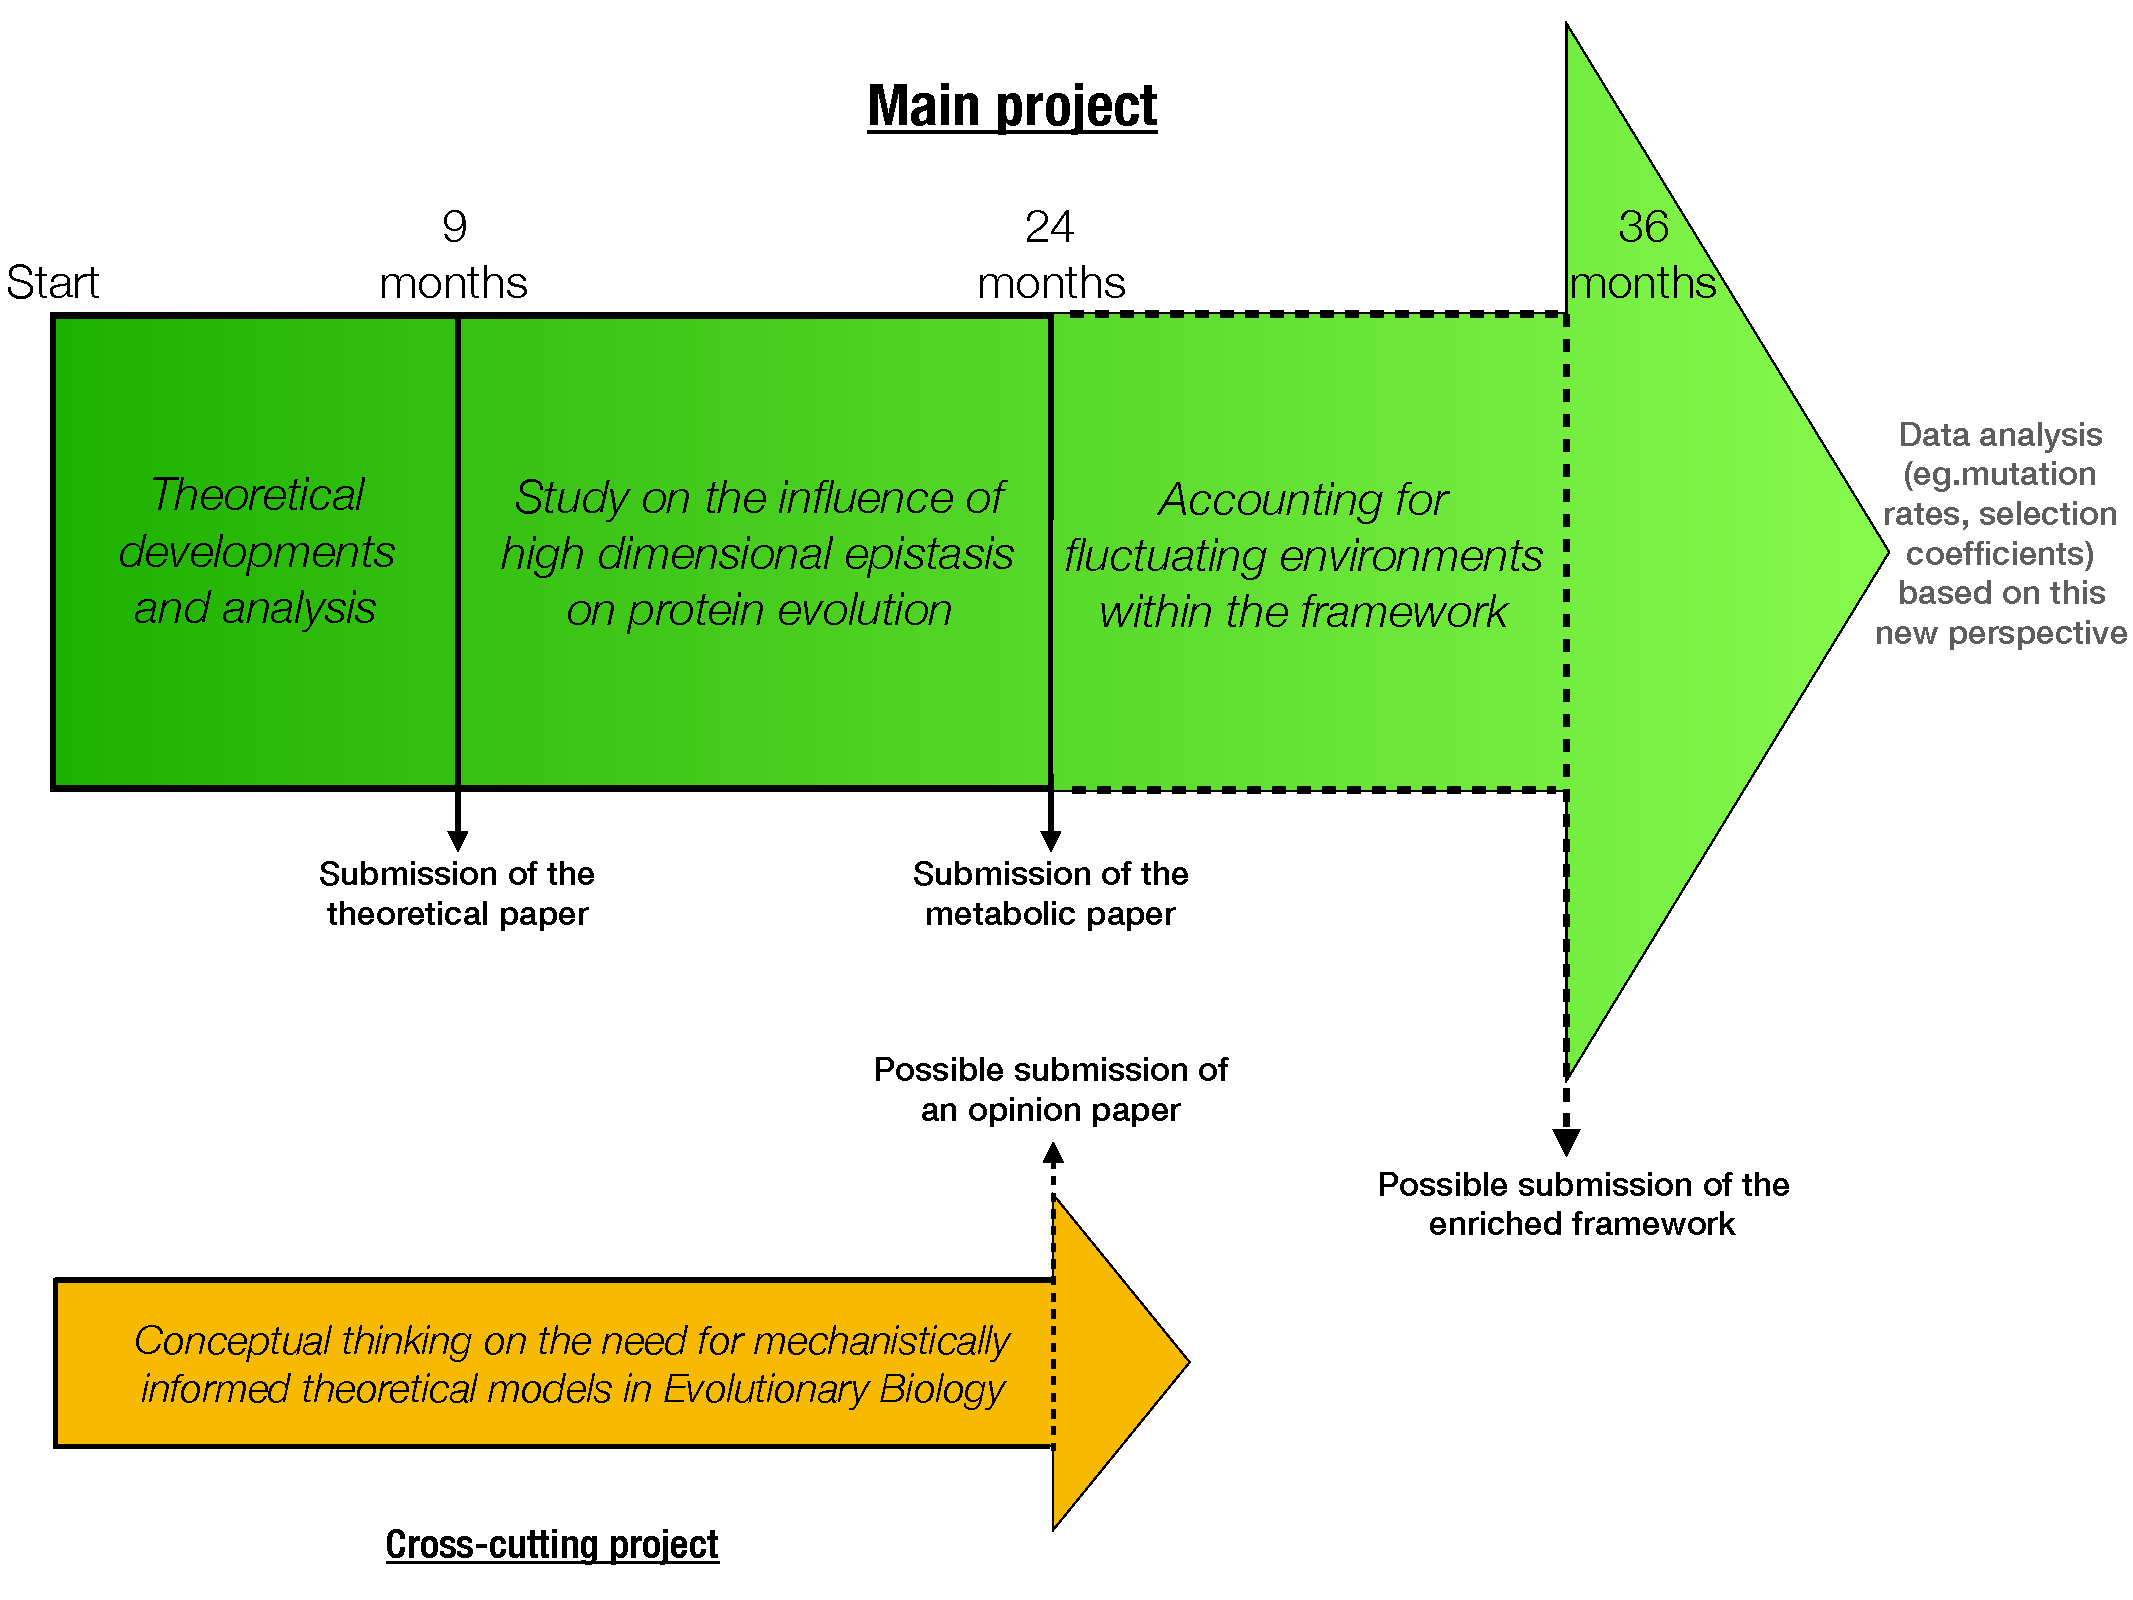
\includegraphics[scale=0.45,trim=0cm 0cm 0cm 0.5cm,clip]{Chronological-PostDoc.pdf}
    \caption{Proposed schedule for the project: the green arrow details a possible roadmap for a research project funded for 24 to 36 months while the gold arrow introduces the possibility of an opinion paper making the case for the development of theoretical population genetics and evolutionary models with more biologically realistic underlyings.}
    \label{fig:ChronologicalTiming}
\end{figure}

\subsection{Possible host laboratories}

Among several others, three laboratories match with the needs and aspirations of this cross-sectional line of research and could possibly be interested by it:
\begin{itemize}
    \item the MacCandlish lab, whose main line of research focuses both on predicting the proximal effect of mutations and how they influence different biological processes;
    \item the Serohijos lab, which intends to combine biophysics, evolutionary biology and population genetics to address fundamental questions in Evolution.
    \item the Weinreich lab, which studies how genetic novelty fuels Evolution using experiments and theoretical approaches.
\end{itemize}

%\bibliographystyle{natbib}%%%%natbib.sty
\bibliography{enzyme.bib}%%%refs.bib

\pagebreak

\section*{APPENDIX: Simulation outcomes for $N_e=10$}

\begin{figure}[h!]
    \centering
    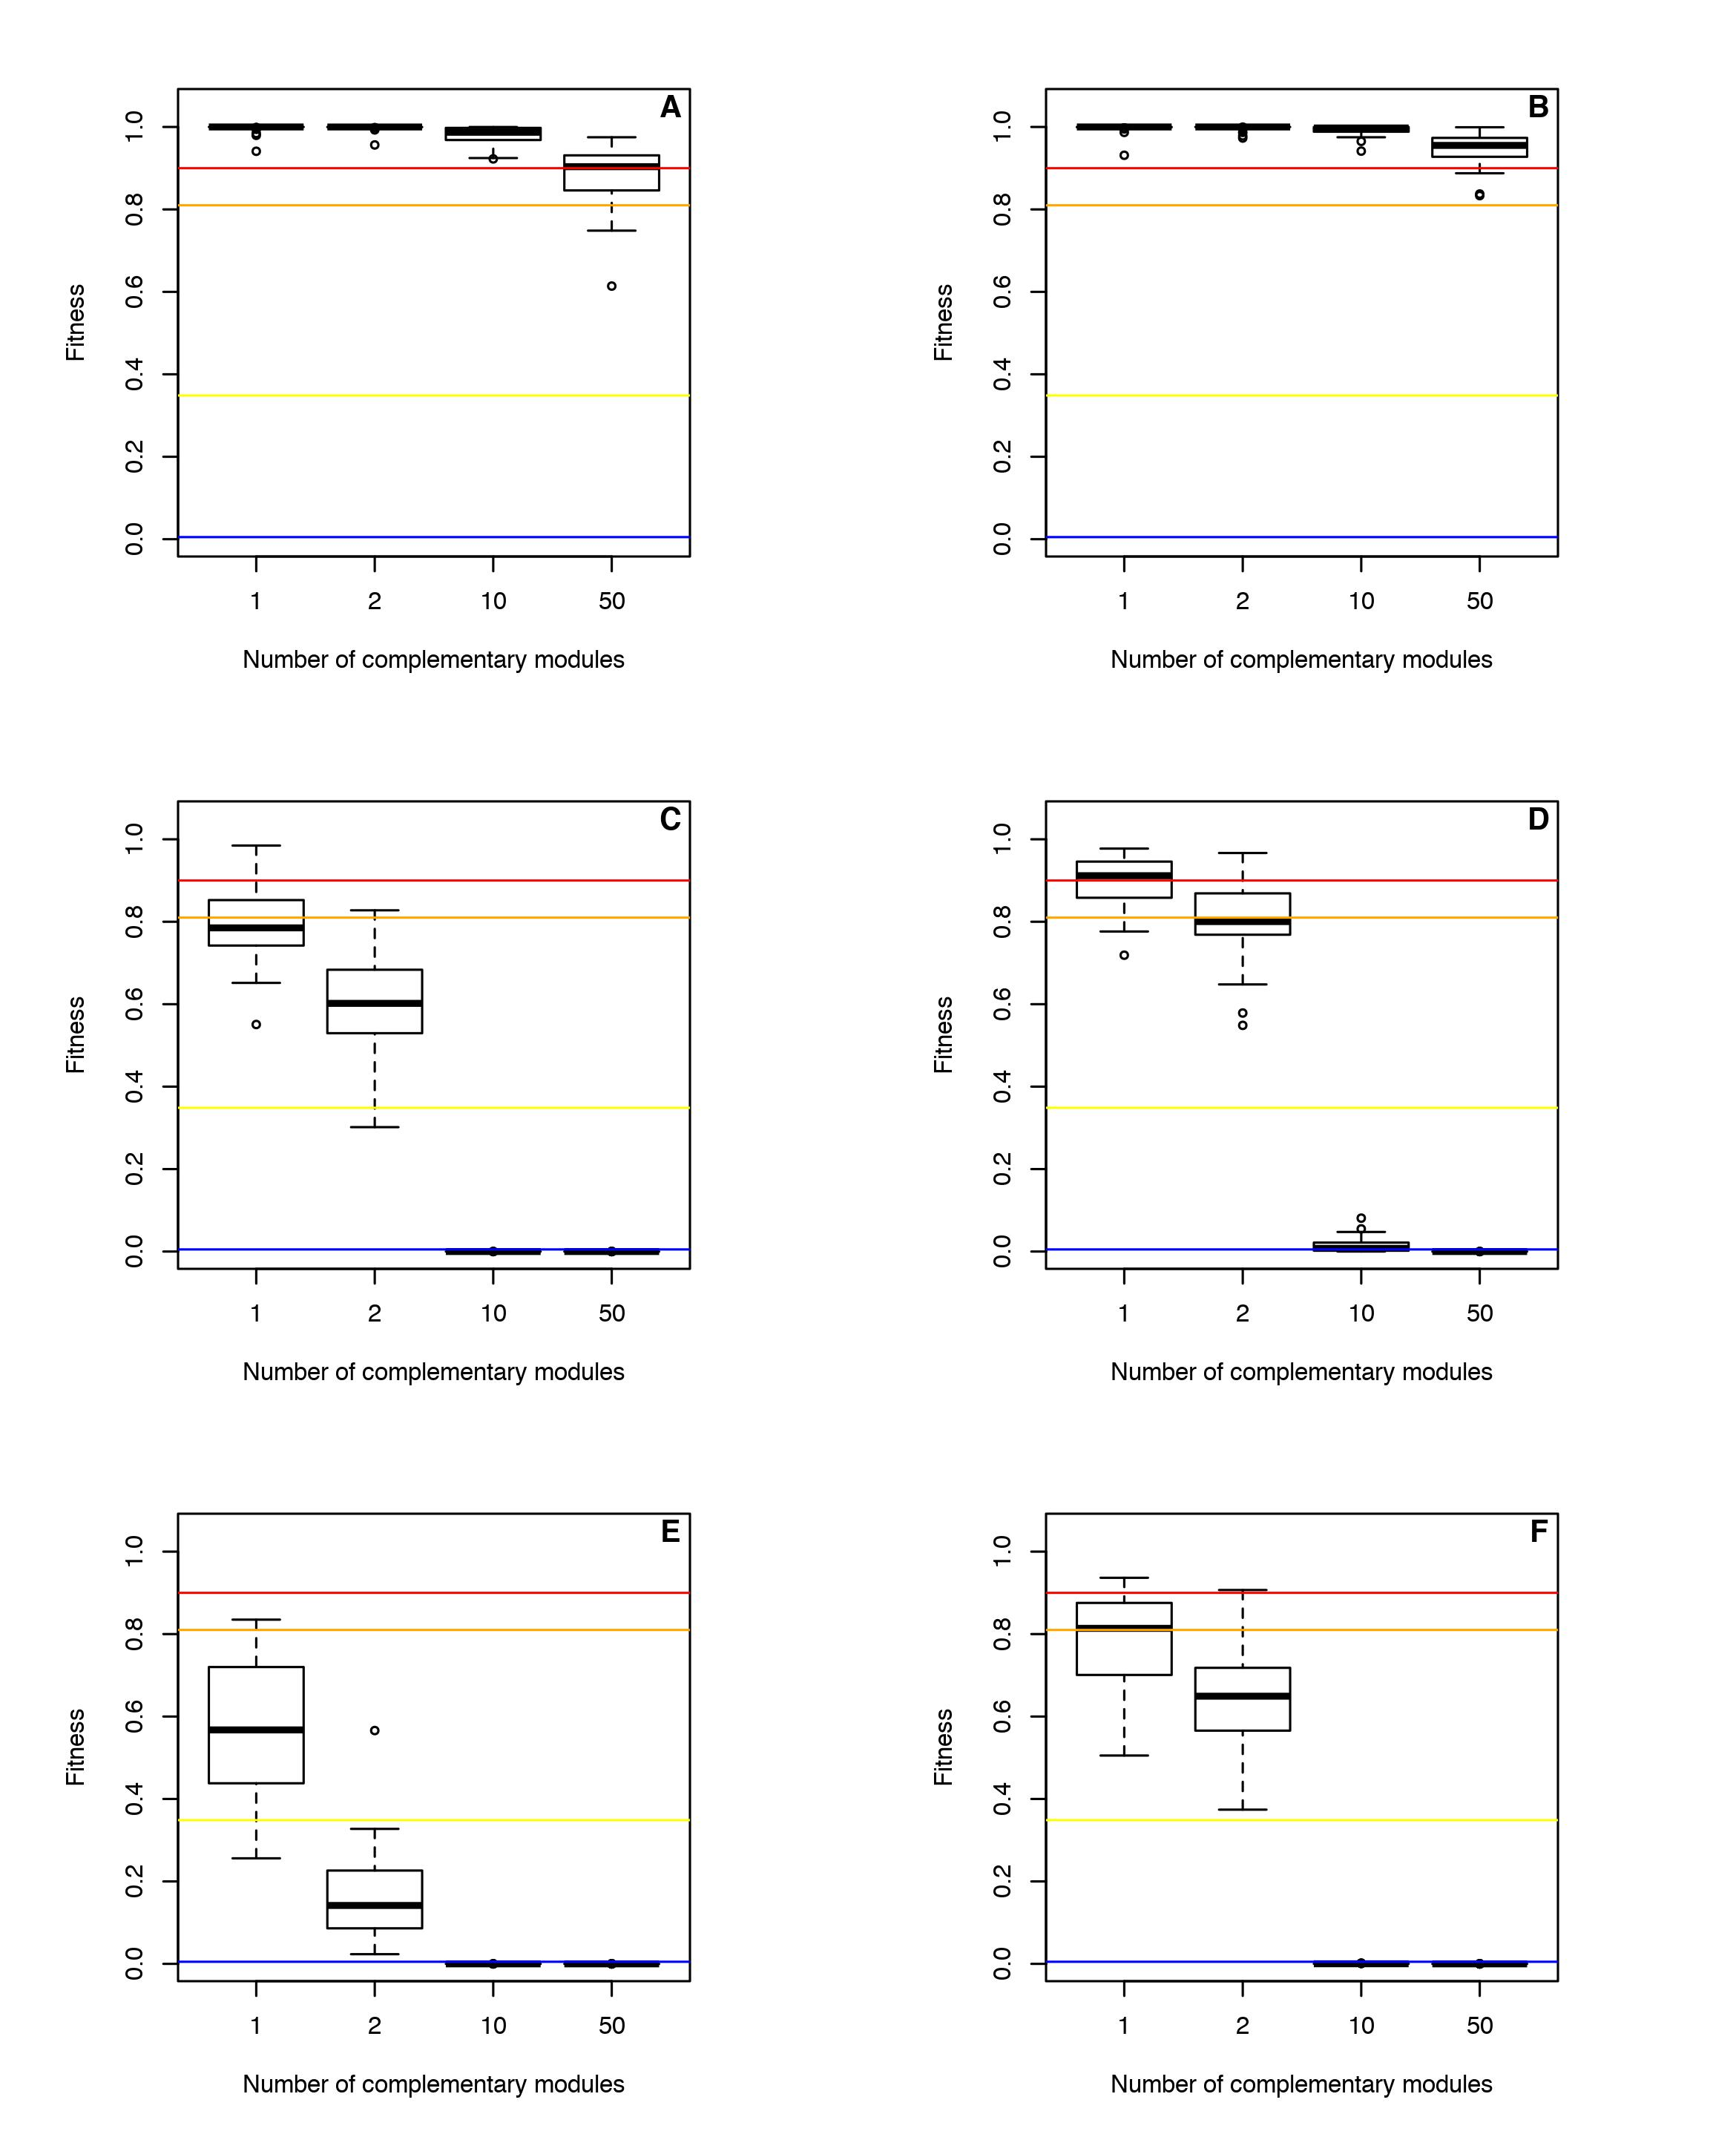
\includegraphics[scale=0.75,trim=0cm 0cm 0cm 0cm,clip]{Evo_Outcomes_Ne10.jpeg}
    \caption{Simulation outcomes for the mutation-election-drift balance with $N_e=10$ when the interplay of complementary epistasis and diminishing returns epistasis (through the fitness landscape of traits) are accounted for. The number of complementary modules varies from 1 to 50. Each line corresponds to a level of mutational bias: null in (A) and (B), low in (C) and (D), high in (E) and (F) - see text for details; each column represents a level of mutational variability, with (A), (C) and (E) having low variability while (B), (D) and (F) display a moderate to high variability.}
    \label{fig:Outcomes10}
\end{figure}

\end{document}
